\subsection{The basic equivalences \cite{poon}}

\begin{proposition}[Equivalences between rings and preadditive categories]
We have the following equivalences of categories:

\begin{enumerate}
\item The category Ring is equivalent to the category PreCat$_1$.
\item The category Ring$\perp$ is equivalent to the category PreCat$_{Fin}$.
\end{enumerate}
\end{proposition}
\begin{proof}
Let's see each of the mentioned equivalences:

1. We define a functor $G:PreCat_1 \to Ring$ as: $$G(C) = R_C = Mor_C(*,*)$$ here $*$ is the unique object of the category and given $H \in  Mor_{PreCat_1}(C,D)$ and $r \in Mor_{C}(*,*)$: $$G(H)(r) = H(r)$$ We observe that this is well-defined since $H$ is an additive functor and gives a ring homomorphism.

\textbf{$G$ is a functor}

\begin{itemize}
\item It preserves the identity morphism, $G(id_C)(r) = id_C(r) = r$, so that $G(id_C)$ is the identity ring morphism in $R_C$.
\item It preserves composition, if $C,D,E \in Ob(PreCat_1)$ and we have $H:C \to D,H':D \to E$,$r \in R_C$, then $G(H \circ H')(r) = (H \circ H')(r) = (G(H) \circ G(H'))(r)$.
\end{itemize}  

\textbf{$G$ is fully faithful and essentially surjective}

To ease notation, one introduces the inverse functor of $G$, $F:Ring \to PreCat_1$, such that: $$F(R) = C_R$$ where $C_R$ is the preadditive category given by $Ob(C_R) = \{\star\}$ and $Mor C_R = R$ and for a morphism $h \in Mor_{Ring}(R,S)$, $F(h):C_R \to C_S$ is an additive functor given by: $$F(h)(*) = *$$ $$F(h)(r) = h(r)$$ We leave as an exercise to check that $F(h)$ is indeed a functor. 

\begin{itemize}
\item $G$ is full. For any $h \in Mor_{Ring}(R,S)$ we have that $G(F(h)) = G \circ F(h) = h$. 
\item $G$ is faithful. Assume $G(H) = G(J)$. Necessarily, $G,H$ must me equal on $Ob(C) = \{\star\}$. On morphisms: $$G(H) = G(J) \implies \forall r \in R. G(H)(r) = G(J)(r) \implies \forall r \in R. H(r) = J(r)$$ Therefore, we have that $G = H$.
\item $G$ is essentially surjective.  Let $R \in Ob(Ring)$, then $G(F(R)) = R$.
\end{itemize}  

2. We define a functor $G:PreCat_{Fin} \to Ring_{\perp}$ such that: $$G(C) = (R_C,I_C)$$ where $R_C = \oplus_{X,Y \in Ob(C)} Mor_C(X,Y)$ is a ring and $$I_C = \{id_X:X \in Ob(C)\}$$ is a complete set of orthogonal idempotents. The representation of this ring ca be done as in the following figure:  \begin{figure}[H]
\centering
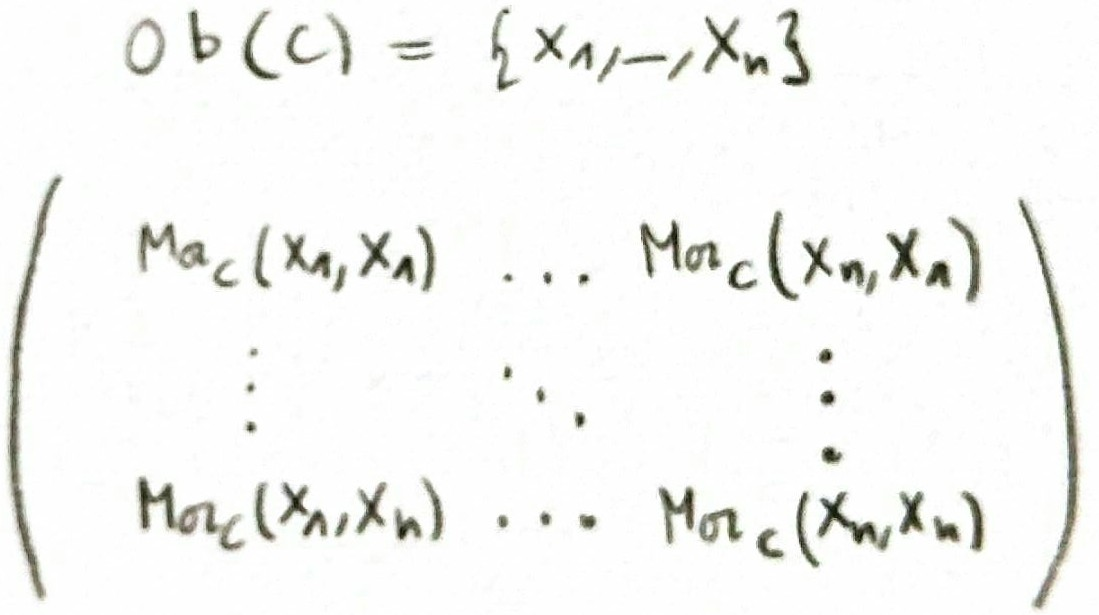
\includegraphics[width=4.5cm]{images/matrix.jpg}
\end{figure} where the order in the indexes is determined for matrix multiplication to compose well the morphisms. The representation of the orthogonal idempotents would be then: \begin{figure}[H]
\centering
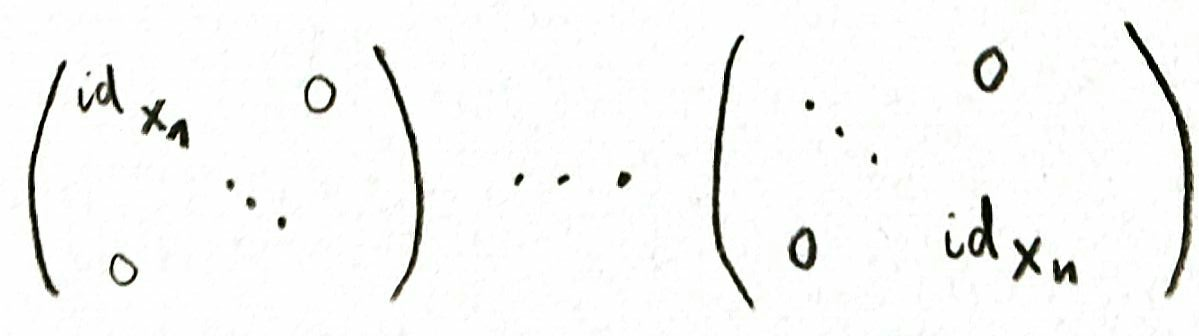
\includegraphics[width=6cm]{images/idem.jpg}
\end{figure}

We leave as an exercise to check that indeed $(R_C,I_C)$ is an idempotented ring. 

Then, for an additive functor $H$ we define: $$G(H)\Big(\sum_{X,Y \in Ob(C)} f_{X,Y}\Big) = \sum_{X,Y \in Ob(C)} H(f_{X,Y})$$ 

\textbf{$G$ is a functor}

\begin{itemize}
\item It preserves the identity morphism since: 

$G(id_C)(\sum_{X,Y} f_{X,Y}) = \sum_{X,Y \in Ob(C)} id_C(f_{X,Y}) = \sum_{X,Y \in Ob(C)} f_{X,Y} = id_{G(C)}(\sum_{X,Y \in Ob(C)} f_{X,Y})$
\item It preserves composition of morphisms since given $C,D,E \in Ob(PreCat_{Fin})$ with morphisms $H:C \to D,H':D \to E$, we have that:

$G(H \circ H')(\sum_{X,Y \in Ob(C)} f_{X,Y}) = \sum_{X,Y \in Ob(C)} H' \circ H(f_{X,Y}) = G(H') \circ  G(H)(\sum_{X,Y \in Ob(C)} f_{X,Y})$.
\end{itemize}

\textbf{$G$ is fully faithful and essentially surjective} 

\begin{itemize}
\item $G$ is full. If $h \in Mor_{Ring_\perp}((R_C,I_C),(R_D,I_D))$ and we take $H \in Mor_{PreCat_{Fin}}(C,D)$ such that: $$H(X) = Dom(h(id_X))$$ $$H(f_{X,Y}) = h(f_{X,Y})$$ In this way, $H(F_{X,Y})$ is a morphism from $H(X)$ to $H(Y)$. So we have: $$G(H)\Big(\sum_{X,Y \in Ob(C)} f_{X,Y}\Big) = \sum_{X,Y \in Ob(C)} H(f_{X,Y}) = \sum_{X,Y \in Ob(C)} h(f_{X,Y}) = h\Big(\sum_{X,Y \in Ob(C)} f_{X,Y}\Big)$$ and therefore, $G(H) = h$. 

\item $G$ is faithful. If $H,J \in Mor_{PreCat_{Fin}}(C,D)$ and we assume that $G(H) = G(J)$ then, they are the same ring homomorphism and so in particular they are equal on the idempotents $id_X$ but this implies that they are equal on objects since $ id_{H(X)} = H(id_X)  = J(id_X) = id_{J(X)}$ so $H(X) = J(X)$. 

On morphisms, if $f_{X,Y} \in Mor_C(X,Y)$ then if $(f_{X,Y})$ denotes the matrix with zero entries except for position $(X,Y)$ containing $f_{X,Y}$, then $G(H)(f_{X,Y}) = G(J)(f_{X,Y}) \implies H(f_{X,Y}) = J(f_{X,Y})$. As a consequence, $H = J$. 

\item $G$ is essentially surjective.

For this part, one uses the inverse functor $F:Ring \to PreCat_{Fin}$ such that for $(R,I) \in Ring_{\perp}$ gives: $$F(R) = C_{(R,I)}$$ where $C_{(R,I)}$ is the category with $Ob(C_{(R,I)}) = I$ and $Mor_{C(R,I)}(e_i, e_j) = e_jRe_i$ and for $h \in Mor_{Ring_{\perp}}((R,I),(S,J))$ we have $F(h)$ defined as: $$F(h)(e_i) = h(e_i)$$ for $e_i \in Ob(C_{(R,I)})$ and for $e_ire_j \in Mor_{C_(R,I)}(e_i,e_j)$: $$F(h)(e_jre_i) = h(e_jre_i)$$ we leave as an exercise to show that $F$ is a functor. 

The strategy then to prove essential surjectivity is, given $(R,I) \in Ob(Ring_{\perp})$ where $I = \{e_1,\ldots,e_n\}$ we claim that $G(F(R)) = G \circ F(R) \cong (M_n(R),I_{M_n(R)}) \cong (R,I)$. The second isomorphism is evident an has been presented above. The first isomorphism uses $\phi:(M_n(R),I_{M_n(R)}) \to G(F(R))$ given by $\phi((e_jre_i)) = (\sum_{i,j} e_jre_i)$.
\end{itemize}

\end{proof}

\begin{exercise}[Proposed to the reader]
If we remove the condition of finite number of objects and we generalize the above construction then we would get infinite matrices:

\begin{figure}[H]
\centering
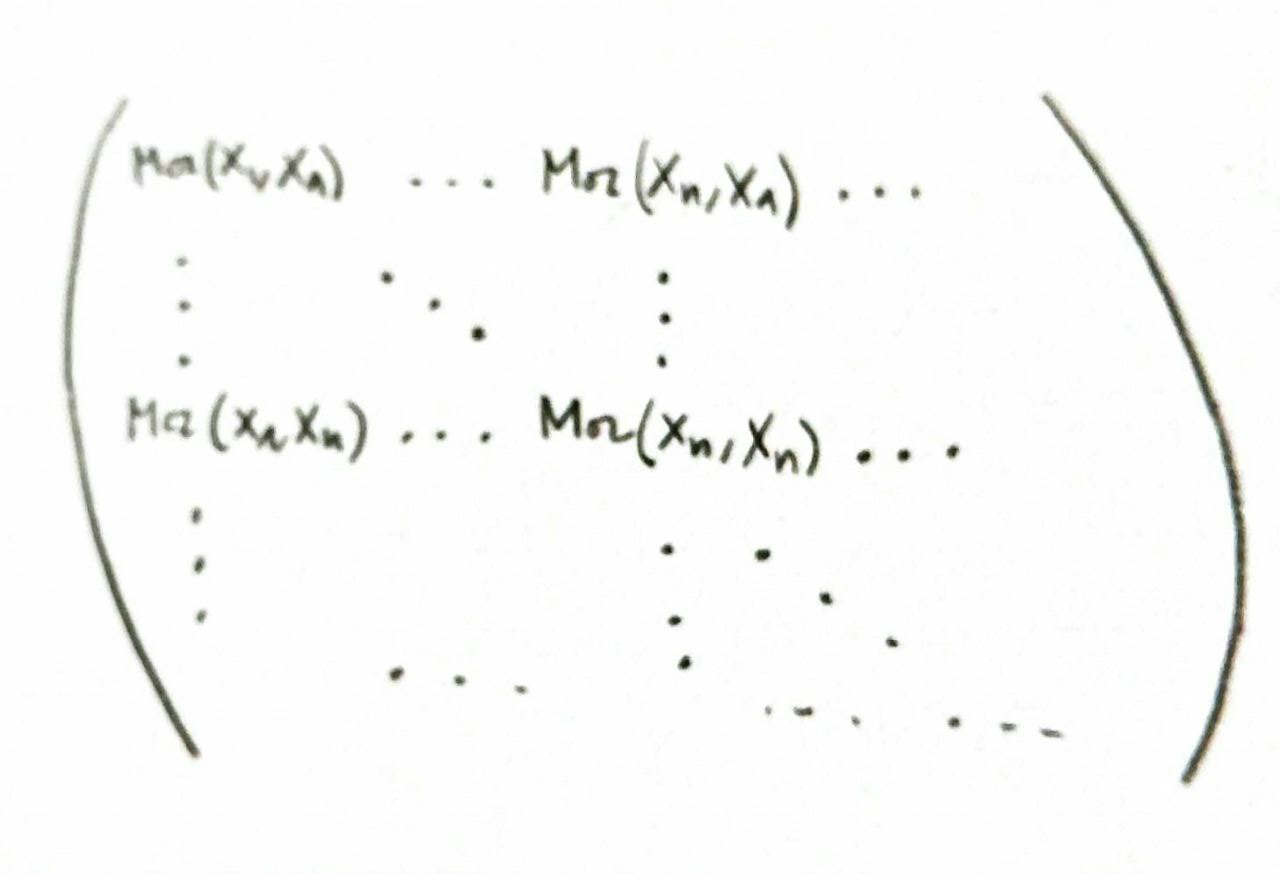
\includegraphics[width=5cm]{images/infinite.jpg}
\end{figure}


that would not have a one (since direct sum has a finite number of non-zero entries):

\begin{figure}[H]
\centering
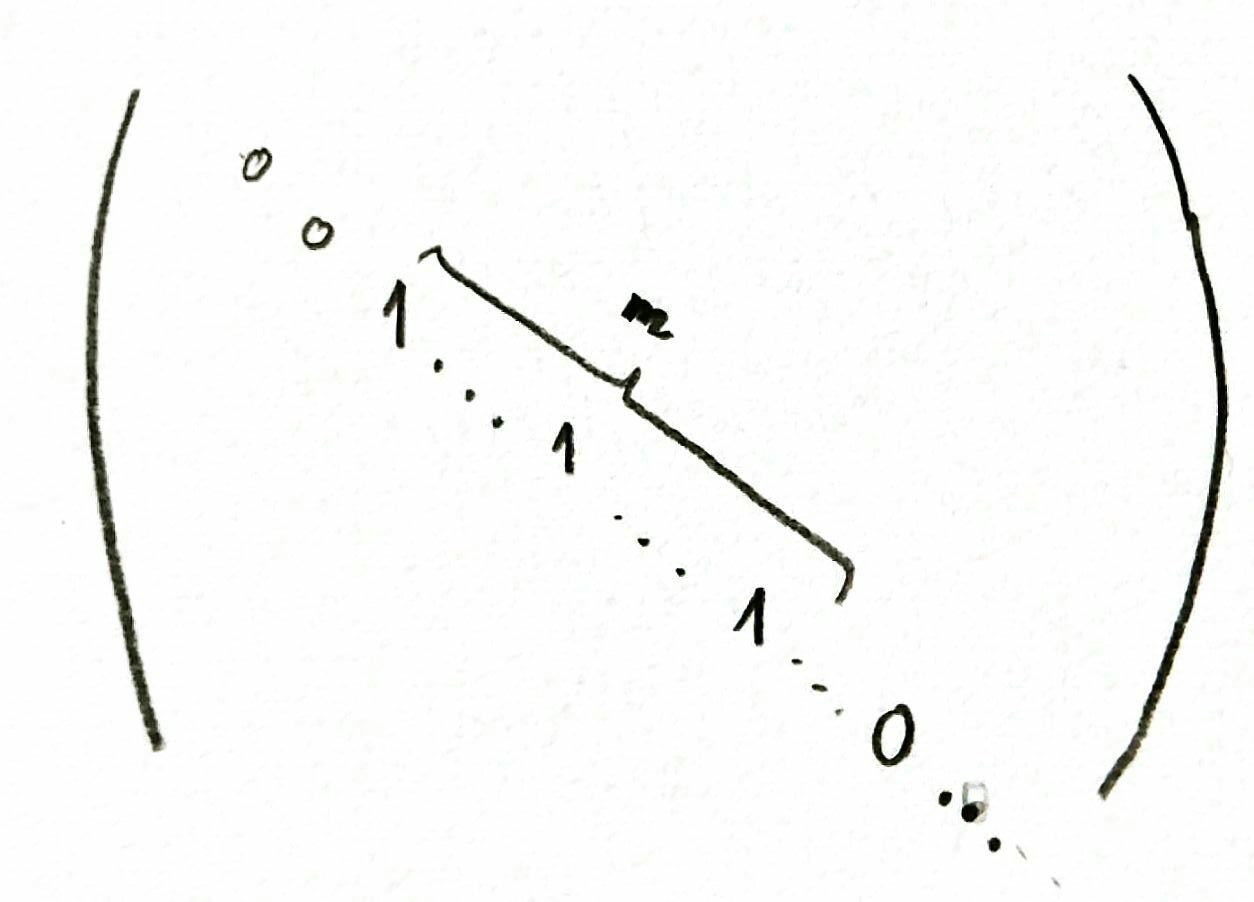
\includegraphics[width=4cm]{images/one.jpg}
\end{figure}

As an exercise, we propose to reader to check if there is an equivalence with rings without one and preadditive categories with an infinite number of objects. 
\end{exercise}

\begin{exercise}[Proposed to the reader]
Can you think of any categorical notion preserved under the equivalences preserved above?

Does this notion provide us with useful theorems about rings, categories or their correspondences?
\end{exercise}

\subsection{Derived results}


\begin{proposition}
Let $(R,I)$ be an idempotented ring that contains no zero divisors and where $Char(R) \neq 2$. Then:

$C_{(R,I)}$ is idempotent complete if and only if $I$ is a complete set of primitive orthogonal idempotents.
\end{proposition}
\begin{proof}
$\implies$ We consider the category $C_{(R,I)}$ as above. We assume that it is idempotent complete. Since we know that $(R,I)$ is an idempotented ring we just have to prove that any non-zero idempotent in $I$ cannot be written as the sum of two non-zero idempotents (not necessarily in $I$). 

Suppose that $e_i = e'+e'' \in I$ where $e',e'' \in I$.  We have to prove that either $e' = 0$ or $e'' = 0$. 

\textbf{$e'$ and $e''$ are pairwise orthogonal}

$e_i = e_i^2 \implies e'+e'' = (e'+e'')^2 = (e'+e'')(e'+e'') = e'e'+e'e''+e''e'+e''e'' = e'+e'e''+e''e'+e''$

$\implies 0_R = e'e''+e''e' \implies e'e''=-e''e' \implies e'e'' = e'e'e''=-e'e''e' \implies e'e''+e'e''e' = 0_R \implies$

 $e'e''(1+e') = 0_R$

Now, since $Char(R) \neq 2$, $(-1)$ is not an idempotent, which implies that $e'e'' = 0_R$. As we wanted. 

\textbf{e'' = 0}

$e'e_ie' = e'(e'+e'')e' = e'e'e'+e'e''e' = e'$ since $e'e'' = 0$. Then, $e_ie'e_i$ is an idempotent as $e_ie'e_i = (e'+e'')e'(e'+e'') = e'$. 

Using that $C_{(R,I)}$ is idempotent complete, we show that, $e_ie'e_i$ is a split idempotent. Indeed, $\exists e_jre_i \in Mor_{C(R,I)}(e_i,e_j),e_ise_j \in Mor_{C(R,I)}(e_j,e_i).e_j = (e_re_i)(e_ise_j) = e_jre_ise_j,e' = e_ie'e_i = (e_ise_j)(e_jre_i) = e_ise_jre_i$. Then we have that:

$e' = e_ise_jre_i =(e'+e'')se_jr(e'+e'') \implies e' = e'e'e' = e'(e'+e'')se_jr(e'+e'')e' = e'se_jre' \implies e'e_ie' = e'se_jre' \implies e'e_ie' - e'se_jre' = 0_R \implies e'(e_i-se_jr)e' = 0_R$

Since $R$ has no zero divisors and $e'$ is nonzero, necessarily, $e_i-se_jr = 0_R \implies e_i = se_jr$. This gives us, $e' = e_ise_jre_i = e_ie_ie_i = e_i$.

Finally, $e_i = e'+e'' \implies e' = e'+e'' \implies e'' = 0_R$. Of course, we have arrived to a contradiction so the implication is complete.

$\Rightarrow$ Assuming $I$ is a complete set of primitive orthogonal idempotents. We take an idempotent morphism $ere \in Mor_{C(R,I)}(e,e)$. We write $e = ere + (e-ere)$ and note that $e-ere$ is an idempotent:

$ \implies (e-ere)(e-ere) = ee - e(ere) - (ere)e + (ere)(ere) = (e-ere)$ 

We have expressed the idempotent $e$ as a sum of two idempotents and since $e$ is in $I$, it is primitive and therefore, $ere = 0$ or $e-ere = 0$. 

If $ere = 0$ then it splits via maps from $0_R$ to $0_R$ ($0$ is an idempotent of the ring). 

If $e-ere = 0$ then $e = ere$ and since $e$ is the identity on $Mor_{C(R,I)}(e,e)$ we can split it as the composition $e \circ e$. 

Therefore, our idempotent $ere$ is a split idempotent and our category is idempotent complete. 
\end{proof}

\begin{exercise}[Proposed to the reader]
Give an interpretation of the above proposition. 

Hint: primitive elements normally imply that decompositions of the ring of the form $R = Re_1 \oplus \ldots \oplus Re_t$ are idecomposable. For instance see the following result taken from \cite{sydney}:

\begin{proposition}
Let $A$ be an $F$-algebra and $e \in A$ an idempotent element. Then $e$ is primitive if
and only if the left ideal $Ae$ is indecomposable.
\end{proposition}

Beware the notions of primitive element may be slightly different!
\end{exercise}

\begin{exercise}[Proposed to the reader]
Does the converse of this proposition hold? That is: 

\begin{proposition}
If $I$ is a complete set of primitive orthogonal idempotents then $(R,I)$ be an idempotented ring that contains no zero divisors and where $Char(R) \neq 2$.
\end{proposition}
\end{exercise}






